\section{Bus Protocol - Design}
\label{sec:bus:design}

According to requirement \ref{req:ulftrtp:interfacing} we segmented the ULFTRTP in independent layers arbitrarily exchangeable with respect to the below defined interfaces.\\

We will see in the subsequent sections the protocols CNI (Communication Network Interface) is considered as a stand alone component with push and pull interfaces.
As this is not always the case the overall control mechanisms of the protocol can slightly vary depending on the platform used.\\

An overview of the protocols design is given in figure \ref{fig:bus:design:overview}. In the following sections parts of the protocol design are considered with more detail.

\begin{figure}[h]
\centering
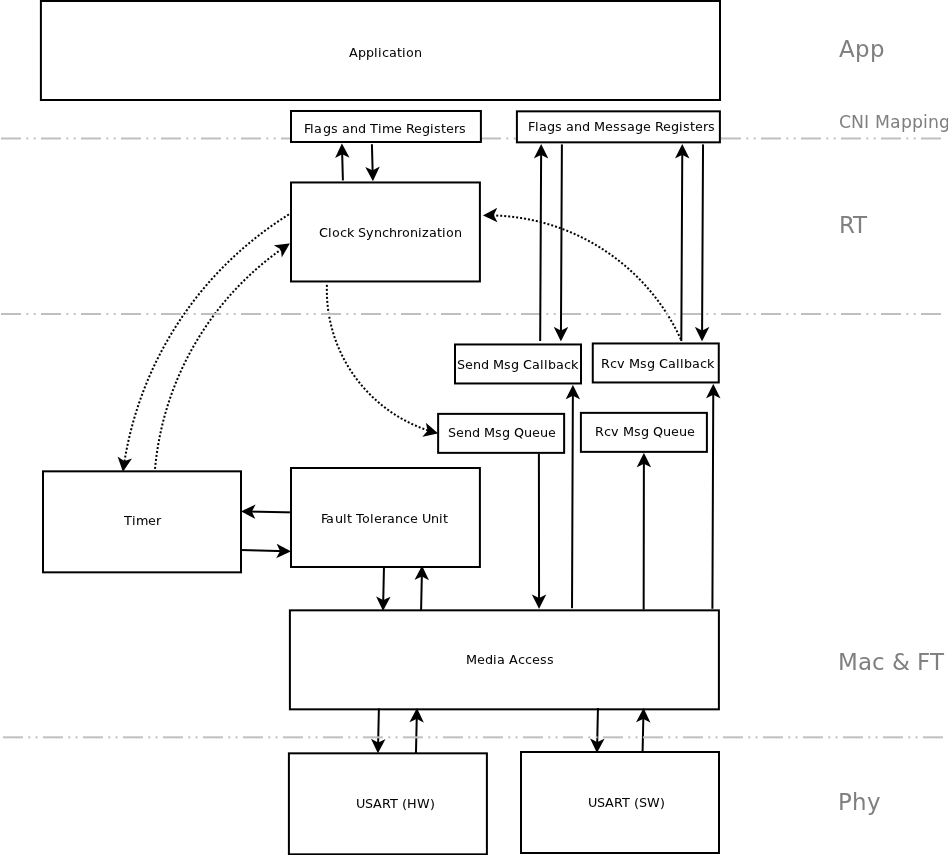
\includegraphics[width=0.8\textwidth]{../images/protocol_design_overview.png}
\caption{Protocol design overview.}
\label{fig:bus:design:overview}
\end{figure}

\subsection{physical access layer}
\label{sec:bus:design:layer1}

The physical layer in the ``ES2011'' configuration is provided by a one-wire-USART terminated with a pull-down resistor, 
leading us to the fact, of a dominant 0 and an recessive 1 level.\\

Since this must not be true for all possible configuratoins supported by the protocol this leads
us to the first physical layer description. To accomplish support for other configurations the physical 
layer provided here has to be adjusted or completely exchanged by specific implementations.\\


\begin{figure}[h]
 \label{fig:bus:design:layer1:usartconfig}

\begin{center}


\definecolor{bgblue}{rgb}{0.41961,0.80784,0.80784}%
\definecolor{bgred}{rgb}{1,0.61569,0.61569}%
\definecolor{fgblue}{rgb}{0,0,0.6}%
\definecolor{fgred}{rgb}{0.6,0,0}%
%
\begin{tikztimingtable}[
    %timing/slope=0,         % no slope
    timing/coldist=2pt,     % column distance
    timing/lslope=0.1,
    xscale=2.05,yscale=2., % scale diagrams
    semithick               % set line width
  ]
  \scriptsize timing  	& 11{C}                              \\
  \scriptsize data                     & .5H L{S} 8D{8Bit} H       \\
  %R                     & [fgblue]  UH .8U 1.4H 0.8L \\
  %MISO & D{z} 2D{z} \\
  %Q                     &          L .8H 1.7L 1.5H LL       \\
  %$\overline{\mbox{Q}}$ &          H .8L 1.7H 1.5L HH       \\
  %Q                     & [fgred]  HLHHHLL                  \\
  %$\overline{\mbox{Q}}$ & [fgred]  LHLLLHH                  \\
\extracode
 \makeatletter
  \begin{pgfonlayer}{background}
%   % Draw shaded backgrounds
%   \shade [right color=bgblue,left color=white]
%      (7,-8.45) rectangle (-2,-4.6);
%   \shade [right color=bgred,left color=white]
%      (7,-12.8) rectangle (-2,-8.6);
  % Add background grid lines
  \begin{scope}[gray,semitransparent,semithick]
    \horlines{}
    \foreach \x in {1,...,10}
      \draw (\x,1) -- (\x,-2); %-12.8
    % similar: \vertlines{1,...,6}
  \end{scope}
  % Add labels
%   \node [anchor=south east,inner sep=0pt]
%     at (7,-8.45) {\tiny clocked};
%   \node [anchor=south east,inner sep=0pt,fgred]
%     at (7,-12.8) {\tiny positive edge triggered};
 \end{pgfonlayer}
\end{tikztimingtable}%

\end{center}

\caption{Timing of 8N1 USART Config.}
\end{figure}

For data transmission we use a USART configuration with 1 start-bit, 
8 data bits, 1 stop bit and no parity, as depicted in Figure 
\ref{fig:bus:design:layer1:usartconfig} \nameref{fig:bus:design:layer1:usartconfig}.
The physical layer as defined in our protocol has to support collission avoidance 
strategies of higher layers, and thus provide mechanisms for bitwise arbitration as described below.\\

To provide bit wise arbitration we need to access the bus 
in the startup-phase of a message in a modified soft-usart.
After the bus is assigned to certain node the communication over the 
hardware supported usart can be established, since this decreases the processor load immensely.


\begin{figure}[h]
 \label{fig:bus:design:layer1:arbitration}

\begin{center}


\definecolor{bgblue}{rgb}{0.41961,0.80784,0.80784}%
\definecolor{bgred}{rgb}{1,0.61569,0.61569}%
\definecolor{fgblue}{rgb}{0,0,0.6}%
\definecolor{fgred}{rgb}{0.6,0,0}%
%
\begin{tikztimingtable}[
    %timing/slope=0,         % no slope
    timing/coldist=2pt,     % column distance
    timing/lslope=0.1,
    xscale=2.05,yscale=2., % scale diagrams
    semithick               % set line width
  ]
  \scriptsize node1  	& HLHHHLHHLHHLLLLH  \\
  \scriptsize node2     & HLHHHLHHLHHLHHHH  \\
  \scriptsize bus       & HLHHHLHHLHHLLLLH  \\
  %R                     & [fgblue]  UH .8U 1.4H 0.8L \\
  %MISO & D{z} 2D{z} \\
  %Q                     &          L .8H 1.7L 1.5H LL       \\
  %$\overline{\mbox{Q}}$ &          H .8L 1.7H 1.5L HH       \\
  %Q                     & [fgred]  HLHHHLL                  \\
  %$\overline{\mbox{Q}}$ & [fgred]  LHLLLHH                  \\
\extracode
 \makeatletter
  \begin{pgfonlayer}{background}
%   % Draw shaded backgrounds
%   \shade [right color=bgblue,left color=white]
%      (7,-8.45) rectangle (-2,-4.6);
%   \shade [right color=bgred,left color=white]
%      (7,-12.8) rectangle (-2,-8.6);
  % Add background grid lines
  \begin{scope}[gray,semitransparent,semithick]
    \horlines{}
    \foreach \x in {1,...,15}
      \draw (\x,1) -- (\x,-4); %-12.8
    % similar: \vertlines{1,...,6}
  \end{scope}
  % Add labels
   \node [anchor=south east,inner sep=0pt]
     at (14.5,-2.5) {\tiny collission detected};
%   \node [anchor=south east,inner sep=0pt,fgred]
%     at (7,-12.8) {\tiny positive edge triggered};
 \end{pgfonlayer}
\end{tikztimingtable}%

\end{center}
\caption{Collission avoidance via arbitration.}
\end{figure}

The arbitration as depicted in figure \ref{fig:bus:design:layer1:arbitration} \nameref{fig:bus:design:layer1:arbitration}
is realized via the soft-usart driver. 
When a node decides to send a message he/she lays the MessageID, 
the ReceiverNodeID and the SenderNodeID bitwise on the bus and reads it back.\\

Since any other node deciding to send a message at the same instant in time, 
has to perform the same collission detection strategie the nodes with a weaker 
arbitration mask detect that the signal on the bus is not the signal driven by themselves.
A node detecting such a behaviour has to switch in a reading state 
at a higher layer leading to only one node accessing the bus exclusively.\\

As briefly mentioned the switch of the arbitration mode to a reading 
mode has to be done on higher layers, it has also to be guaranteed 
by higher layers that during reading a message the node must not write data to the bus.


\subsection{Media access and fault tolerance layer}
\label{sec:bus:design:layer2}

The second layer of our protocol can be seen as a composition of two internal layers, 
namely the media access sublayer controlling the basic bus access as depicted in section 
\ref{sec:bus:basicaccess} \nameref{sec:bus:basicaccess} and the state machine defining 
the communication process and the fault tolerant sublayer providing basic fault 
tolerant mechanisms like the starvation handling (see section \ref{sec:bus:ftnsh}).\\

% These two sublayers and their interactions are described in the sections 
% \ref{sec:bus:design:layer2:mac} \nameref{sec:bus:design:layer2:mac} and 
% \ref{sec:bus:design:layer2:ft} \nameref{sec:bus:design:layer2:ft} in detail. 
In the following section we describe the general workflow of the MAC \& FT layer.

\subsubsection{General workflow}
To describe the general workflow of the MAC \& FT layer we examine how messages are sent and received.\\

\paragraph{Transmission of messages}
When a higher layer (including the application) wants to send a message it adds the message to the \textit{Send Msg Queue} which is provided
by a ring buffer holding all the messages payloads and the messages types. The highest prior message is stored in the protocols state machine, waiting for the bus to be free.\\

When the bus seems to be free, e.g. the transmission of a previous message has completed, the protocol tries to arbitrate the bus via the message type delivered through the message description held in the queue.\\

If the arbitration was successful the rest of the message is transmitted and the next message from the queue is fetched into the protocols finite state machine. Otherwise the message is kept in the finite state machine of the protocol and retransmitted when the bus is free again.
Whenever there was a transmission attempt whether successful or not a callback routine is fired propagating the current status of the protocol to higher level layers or to the flags and registers separating the application from the communication network interface.\\

\paragraph{Reception of messages}
When the USART reports the reception of data the protocol changes in a receiving state in which it is not allowed to transmit data.
Whenever data is receipt by the USART the fault tolerant non starvation protocol resets the timer providing basic error detection in the time domain.\\

When the timer triggers an interrupt the node knows that the transmitting node has timed out and that it can change in an idle state or transmit its own messages.\\

When a message is completely received its integrity is checked trough the CRC checksum and the message is added to the \textit{Receive Message Queue} and a \textit{Receive Callback} is triggered, informing higher level layers of the data receipt and updating the registers and flags of the CNI mapping.

%\subsubsection{Mac \& FT layer interface}
\label{sec:bus:design:layer2:interface}

The Mac \& FT layer  provides its interfaces in such a way as it takes only data via methods and returns data only via callback routines (which can be seen as events).\\

The methods provided by the interface are

\begin{enumerate}
 \item \textbf{initialize: } initializes the layer and triggers the initialization of the sublayers it uses.
 \item \textbf{writeMessage: } takes an arbitrary message payload and the payloads size in bytes, appends it to the \textit{send queue} and triggers the transmission of the next message in the queue.
 \item \textbf{writeMessageImmediate: } takes an arbitrary message payload and the payloads size in bytes, inserts it at the next position to be read in the \textit{send queue} and triggers the transmission of the next message in the queue.
\end{enumerate}

and the events provided by the interface are

\begin{enumerate}
 \item \textbf{messageReceivedCallback}
 \item \textbf{messageTransmittedCallback}
 \item \textbf{queueOverflowCallback}
\end{enumerate}










The workflow of the layers statemachine is depicted in figure \ref{fig:bus:design:layer2:statemachine} and starts in the state \textit{STARTUP}, in which a state ``synchronzies'' to the bus.

After this process the statemachine changes to state \textit{IDLE}.
When a message is appended to the queue in state \textit{IDLE} the CRC of the message is calculated and the transmission is started (\textit{SND\_ARBITRATION}) by trying the bus arbitration.\\

After the arbitration was done successfully the remaining message is transmitted in the state \textit{SND\_DATA/CRC} and the event \textit{messageTransmittedCallback} is triggered, otherwise the meanwhile received/sent data is handed out to the receive procedure and the state \textit{RCV\_ARBITRATION} is reached in which messages sent by other communication partners are received.\\

When an arbitration of another node is detected in state \textit{IDLE} the statemachine switches to state \textit{RCV\_ARBITRATION} and the receiving procedure can be done.\\

Whenever a message is successfully received the message is appended to the \textit{recv queue} and the \textit{messageReceivedCallback} event is triggered notifying higher layers of the message arrival.\\

In case the \textit{send queue} or the \textit{recv queue} overflows and data is lost the event \textit{queueOverflowCallback} is triggered to notify higher layers.\\

\begin{figure}[H]
\centering
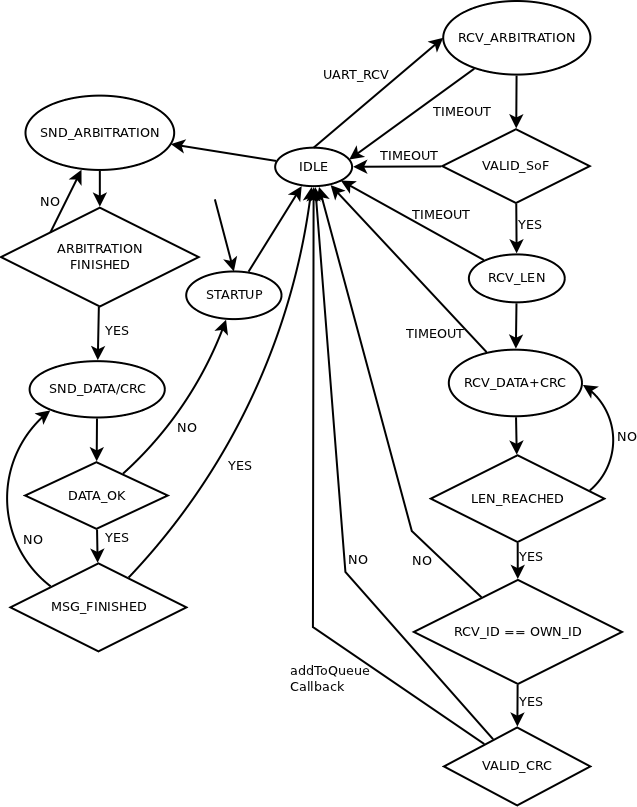
\includegraphics[width=0.8\textwidth]{../images/layer2_state_machine.png}
\caption{Layer2 state machine}
\label{fig:bus:design:layer2:statemachine}
\end{figure}

\subsection{Real time layer}
\label{sec:bus:design:layer3}
\label{sec:bus:design:layer6}
The RT (real time) layer is on top of the MAC \& FT layer described in section \ref{sec:bus:design:layer2} and provides clock synchronization mechanisms to achieve a commonly agreed notion of time within the nodes.\\

In our implementation we will provide a clock synchronization upon an averaging algorithm with acceptable granularity, providing us with a globally agreed sparse time base.\\

To minimize latency and jitter during the timestamping and the evaluation of a synchronization message we bypass the FIFO ordering within the queue and add clock synchronization messages directly to the media access sublayer.\\